\section{Validierungen}

Alle Benutzereingaben werden durch sinnvolle Validierungen überprüft. Diese wurden in den jeweiligen Model-Klassen
für dessen Felder ergänzt. So können nun beispielsweise keine Lösungen ohne Uploads abgegeben werden, keine Kommentare
ohne Inhalt u.v.m.

\begin{codebox}
\begin{minted}{ruby}
class Assessment < ApplicationRecord
  validates :title, :starts_at, presence: true
  validates :duration_in_minutes, presence: true, 
            numericality: { only_integer: true, greater_than: 0 }

  ...
end
\end{minted}
\end{codebox}

Das \enquote{simple\_form} gem nimmt zusätzlich die ganze Arbeit im Frontend ab und stellt die Validierungen in einer Benutzerfreundlichen
Weise dar.

\begin{figure}[H]
  \centering
  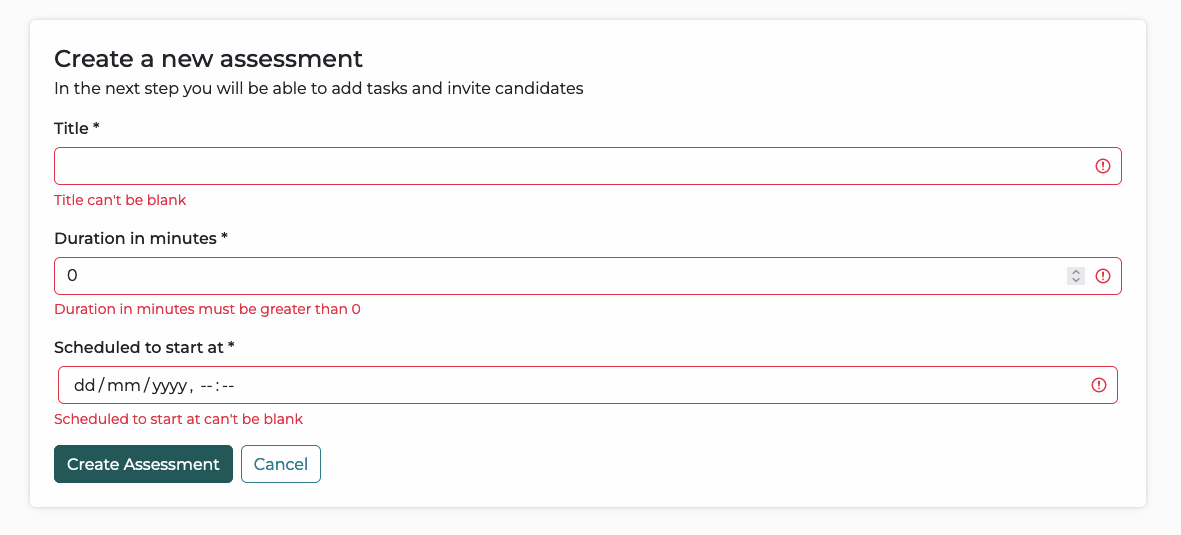
\includegraphics[width=\textwidth]{images/ui/validations.png}
  \caption{\label{fig:validations} Validierungen dargestellt durch das \enquote{simple\_form} gem}
\end{figure}
